\documentclass{standalone}
\usepackage{pgf}
\usepackage{tikz}
\usetikzlibrary{arrows,automata}
\usepackage[latin1]{inputenc}
\begin{document}
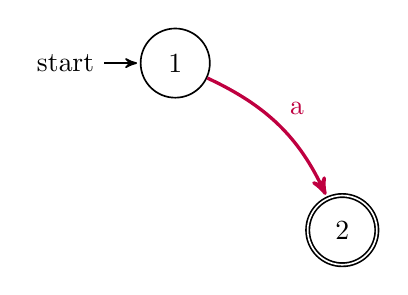
\begin{tikzpicture}
[->,>=stealth',shorten >=1pt,auto,node distance=3.0cm,semithick]\tikzstyle{every state}
=[fill=none,draw=black,text=black]
\node[initial,state] (1) {$1$};
\node[state, accepting] (2) [below right of=1] {$2$};

\path
(1) edge [purple, very thick, bend left=20]  node {a} (2)
;\end{tikzpicture}
\end{document}
